\documentclass{article}
\usepackage{iclr2027_conference,times}
\usepackage[T1]{fontenc}
\usepackage{lmodern}
\input{math_commands.tex}
\usepackage{amsmath,amssymb,amsthm,mathtools,bm,booktabs,microtype,graphicx}
\usepackage[draft]{hyperref}
\usepackage{url}

\newtheorem{theorem}{Theorem}
\newtheorem{lemma}[theorem]{Lemma}
\newtheorem{corollary}[theorem]{Corollary}
\newtheorem{proposition}[theorem]{Proposition}
\newtheorem{definition}[theorem]{Definition}
\newtheorem{remark}[theorem]{Remark}
\newcommand{\one}{\mathbf 1}
\newcommand{\Reg}{\operatorname{Reg}}
\newcommand{\Gap}{\operatorname{Gap}}
\newcommand{\BRGap}{\operatorname{BRGap}}
\newcommand{\range}{\operatorname{range}}
\newcommand{\pos}[1]{\left[#1\right]_+}

\title{Self-Bounding Regret Matching+ in Potential Games\\and Product-Simplex Optimization}

\author{\textbf{Pahan Dewasurendra} \\ Johns Hopkins University}

\hypersetup{pdftitle={Self-Bounding Regret Matching+ in Potential Games and Product-Simplex Optimization},pdfauthor={Pahan Dewasurendra},pdfkeywords={self-bounding, regret, matching, potential, games, product-simplex, optimization, parameter, free},pdfsubject={preprint}}
\begin{document}
\maketitle

\begin{abstract}
Regret matching+ (RM+) is parameter free, scale invariant, and central to large game solving, but its only general individual-regret guarantee grows as $\sqrt{T}$. A recent ICLR result used this envelope to prove that RM+ reaches an $\epsilon$-stationary point of a smooth objective over a product of simplices in $O(\epsilon^{-4})$ iterations, or $O(\epsilon^{-8})$ from the standard zero initialization. We give an exact one-step conservation law for RM+. It states that forward utility gain pays for both squared state motion and growth of the regret-state norm. Norm growth is at most $\sqrt{m-1}$ times forward gain for $m$ actions, and the coefficient is sharp. This yields four results for unmodified RM+. Its regret on any utility path is controlled by centered temporal variation. Its regret is uniformly bounded under alternating play in every finite exact potential game, resolving an open question and making squared activation gaps summable. Both certified lazy and ordinary cyclic play attain an $\epsilon^{-2}$ exponent. On any smooth, possibly nonconcave simplex objective, RM+ finds an $\epsilon$-KKT point in $O(\epsilon^{-2})$ iterations. Most broadly, for a smooth objective over an arbitrary product of simplices, cyclic block RM+ attains the same $O(\epsilon^{-2})$ exponent from arbitrary initialization, with an explicit trajectory-dependent constant. The proof controls the finite objective loss caused by low-state blocks and then self-bounds every block state and the total squared path length. Complete proofs cover zero states, sharpness, common-profile stationarity, and robust gain dominance. Oracle-normalized diagnostics compare RM+ with predictive and smooth extra-gradient variants on graphical potential games and dense nonconvex objectives.
\end{abstract}

\section{Introduction}

Regret matching is a foundational procedure for online learning and adaptive play~\citep{Hart00:Simple}. Its positive-truncation variant, regret matching+ (RM+), is a basic component of counterfactual regret minimization systems that solve very large imperfect-information games~\citep{Tammelin14:Solving,Zinkevich07:Regret}. RM+ is unusually simple. It keeps a nonnegative regret vector, normalizes it to obtain the next mixed strategy, and introduces no learning-rate parameter. Its scale invariance and practical speed have motivated connections to Blackwell approachability and mirror descent, predictive variants, and stabilization schemes~\citep{Farina21:Faster,Farina23:Regret,Cai25:Last,Zhang25:Scale,Meng26:Faster}.

Beyond two-player zero-sum games, however, even qualitative convergence was unresolved until recently. \citet{Anagnostides26:Convergence} proved that RM+ reaches approximate KKT points for smooth optimization over products of simplices. Their result implies convergence to Nash equilibria in potential games, a question open for two decades~\citep{Marden07:Regret,Kleinberg09:Multiplicative}. The analysis gives an $O(\epsilon^{-4})$ rate when every block is initialized above a prescribed threshold and only $O(\epsilon^{-8})$ from standard zero initialization. Its key denominator is the accumulated regret state. If that state were uniformly bounded, their framework would instead give the canonical $O(\epsilon^{-2})$ rate. They explicitly leave open whether RM+ can incur $\Omega(\sqrt T)$ regret in a potential game. The broader optimization benchmarks of \citet{Tewolde26:Decision} show strong empirical RM+ performance. No proof or superconstant example was known.

We prove that constant regret is forced by the RM+ update whenever its forward gains have finite budget. Let $r$ and $r'$ be consecutive nonnegative regret states, let $x$ and $x'$ be their normalizations, and let $u$ be the current utility vector. Define the forward gain $D=\langle x'-x,u\rangle$. Our starting point is the exact identity
\begin{equation}
2\|r'\|_1D=\|r'\|_2^2-\|r\|_2^2+\|r'-r\|_2^2.
\label{eq:identity-intro}
\end{equation}
The squared-motion term underlies the earlier one-step improvement analysis. The first term on the right was discarded there. Retaining it closes the loop because regret itself is bounded by the state norm. In fact, we prove the sharp charge
\begin{equation}
\|r'\|_2-\|r\|_2\le \sqrt{m-1}\,D.
\label{eq:charge-intro}
\end{equation}
The factor $\sqrt{m-1}$ cannot be improved.

Equation~\eqref{eq:charge-intro} gives a pathwise online-learning theorem. For every utility sequence and arbitrary nonnegative initialization,
\begin{equation}
\Reg_T\le \|r_T\|_2\le \|r_0\|_2+\sqrt{m-1}\sum_{t=1}^T\langle x_{t+1}-x_t,u_t\rangle.
\label{eq:path-intro}
\end{equation}
This is a self-bounding guarantee. It does not require the utilities to be stochastic, smooth, or chosen obliviously. Summation by parts immediately bounds the last sum by centered temporal variation. Thus vanilla RM+, without predictions, attains the better of its adversarial square-root guarantee and a first-order variation guarantee whose accompanying state-norm constant is sharp.

The same theorem has stronger consequences when the utility path is generated by optimization or a game. In an exact potential game under sequential unilateral updates, $D_t$ is exactly the increase in the mixed extension of the potential. It is nonnegative, and its sum never exceeds the potential range. Therefore every player's regret is bounded by a horizon-independent constant. This answers the open question for alternating RM+ and improves the $\epsilon$ dependence of both lazy and ordinary cyclic play from four to two. The ordinary bound has a trajectory-dependent $\delta^{-2}$ constant, while a phased lazy variant avoids this constant, is target-free, and always retains a certified approximate Nash profile.

For a smooth objective, the argument is less direct because forward linearized gain need not equal objective improvement. Above an explicit state-norm threshold, smoothness ensures that the objective pays at least half of $D_t$. On one simplex, the finite objective range therefore bounds all subsequent gain, and~\eqref{eq:charge-intro} prevents further state growth. This gives
\begin{equation}
\min_{1\le t\le T}\Gap(x_t)=O(T^{-1/2}),
\end{equation}
where $\Gap$ is the simplex KKT gap. This is an $O(\epsilon^{-2})$ iteration bound for the original parameter-free trajectory.

The main obstacle on a product of simplices is that low-state block updates may decrease the objective and erase high-state ascent. We show that this loss is finite. Before a block crosses its threshold, state monotonicity bounds its squared state motion. A trajectory-dependent lower bound $\delta$ on positive state norms converts this into a finite squared strategy-motion budget, hence a finite smoothness loss. The objective range then bounds all high-state gain. The sharp charge closes a simultaneous system of bounds on every block state and on the global squared path. Finally, smoothness transfers each block's activation-time gap to a common cycle endpoint. For cyclic block RM+ on any smooth product-simplex objective,
\begin{equation}
\min_{1\le k\le K}\Gap_\Pi(x^k)=O(K^{-1/2}),
\end{equation}
with all constants explicit. Thus the $\epsilon$ exponent improves from four to two under prescribed large initialization and from eight to two under zero initialization.

Table~\ref{tab:summary} summarizes the changes. Simultaneous block updates remain outside our general product theorem because their linearized gains need not decompose into sequential objective changes.

\begin{table}[t]
\centering
\small
\begin{tabular}{@{}lll@{}}
\toprule
Setting & Previous guarantee & This work \\
\midrule
Favorable online utilities & $O(\sqrt{mT})$ & $O(\sqrt m\,V_T)$ \\
Alternating exact potential game & $O(\sqrt{mT})$ regret & $O(\sqrt m\,\Delta_\Phi)$ regret \\
$\epsilon$-lazy potential play & $O(\epsilon^{-4})$ sweeps & $O(\epsilon^{-2})$ sweeps \\
Ordinary cyclic potential play & $O(\epsilon^{-4})$ sweeps & $O(\delta^{-2}\epsilon^{-2})$ sweeps \\
Smooth objective, one simplex & $O(\epsilon^{-4})$ iterations & $O(\epsilon^{-2})$ iterations \\
Smooth product, large initialization & $O(\epsilon^{-4})$ cycles & $O(\epsilon^{-2})$ cycles \\
Smooth product, zero initialization & $O(\epsilon^{-8})$ cycles & $O_\delta(\epsilon^{-2})$ cycles \\
\bottomrule
\end{tabular}
\caption{Consequences for unmodified RM+. Here $V_T$ is centered temporal variation, $\Delta_\Phi$ is potential range, and $\delta$ is the first-positive-state quantity defined below. The displayed rates suppress dimension, range, smoothness, and initialization constants. Previous optimization and potential-game rates are from \citet{Anagnostides26:Convergence}.}
\label{tab:summary}
\end{table}

\paragraph{Contributions.} We establish the exact identity~\eqref{eq:identity-intro}, the sharp charge~\eqref{eq:charge-intro}, and a matching construction. We derive a variation-adaptive regret theorem for vanilla RM+. We prove constant regret and summable activation gaps in alternating exact potential games, a certified $O(\epsilon^{-2})$ lazy rate, and an $O(\delta^{-2}\epsilon^{-2})$ ordinary cyclic rate. For smooth nonconvex optimization, we prove $O(\epsilon^{-2})$ KKT rates both on one simplex and, through a new low-state loss budget, on arbitrary products under cyclic block updates. The proofs are deterministic and preserve the parameter-free, scale-invariant update.

\paragraph{Related work.} RM and RM+ arise from Blackwell approachability and can be viewed as FTRL and Euclidean OMD on the positive orthant~\citep{Hart00:Simple,Farina21:Faster}. Predictive RM+ can be unstable, motivating restarted, clipped, smooth, and extra-gradient variants~\citep{Farina23:Regret,Cai25:Last,Meng25:Smooth}. \citet{Zhang25:Scale} obtain constant regret under a weighted Minty condition for their modified extra-gradient IREG-PRM+ algorithm. \citet{Meng26:Faster} modify smooth predictive RM+ through adaptive regret domains. In contrast, our results concern vanilla nonpredictive RM+ and use favorable realized forward gain rather than an RVU inequality. \citet{Dorazio21:Optimistic} give prediction-sensitive Lagrangian-hedging bounds, including a path-length result for an optimistic RM+ variant on a fixed smooth loss. Variation-dependent regret more broadly has a long history in online learning~\citep{Hazan10:Variation,Chiang12:Gradual}. Those results design regularized-leader or modified gradient and multiplicative-weight methods around gradual variation. Our centered temporal-variation result changes neither RM+ nor its feedback.

Near-constant or constant regret is known for other dynamics under different structures. These include paced optimistic FTRL in general games, adaptive scale-invariant FTRL in zero-sum games, extrapolated FTRL in harmonic games, and optimistic fictitious play in two-action zero-sum games~\citep{Soleymani25:Cautious,Tsuchiya26:Scale,Legacci24:Harmonic,Lazarsfeld25:Optimism}. These algorithms use optimism, regularization, adaptive pacing, or best responses. Conversely, \citet{Anagnostides26:FTRL} prove exponential convergence lower bounds for broad permutation-invariant FTRL dynamics in two-player potential games, and doubly exponential bounds for fictitious play with many players. RM+'s orthant truncation creates the different self-bounding mechanism studied here. Recent fast statistical rates for KL-regularized $\alpha$-potential games concern offline estimation under reference-anchored coverage, not iteration complexity of unmodified RM+~\citep{Chen26:Offline}. Discounted regret matching deliberately bounds old regret through forgetting~\citep{Brown19:Discounted}. We show that no forgetting is needed in exact potential games because forward gain itself pays for state growth. Earlier potential-game dynamics either change regret aggregation or analyze different learning rules~\citep{Marden07:Regret,Kleinberg09:Multiplicative}. The closest work is \citet{Anagnostides26:Convergence}, whose one-step inequality and ascent region we sharpen and close.

\section{RM+ and its exact conservation law}
\label{sec:identity}

For $m\ge2$, write $\Delta_m=\{x\in\mathbb R_+^m:\langle x,\one\rangle=1\}$. RM+ begins with $r_0\in\mathbb R_+^m$. If $r_{t-1}\ne0$, it plays $x_t=r_{t-1}/\|r_{t-1}\|_1$. At the origin it plays an arbitrary fallback. After observing $u_t\in\mathbb R^m$, it sets
\begin{equation}
g_t=u_t-\langle x_t,u_t\rangle\one,
\qquad
r_t=\pos{r_{t-1}+g_t}.
\label{eq:update}
\end{equation}
The next strategy is $x_{t+1}=r_t/\|r_t\|_1$ if $r_t\ne0$. If $r_t=0$, retain $x_{t+1}=x_t$. Let $s_t=\|r_t\|_1$, $R_t=\|r_t\|_2$, $q_t=r_t-r_{t-1}$, and
\begin{equation}
D_t=\langle x_{t+1}-x_t,u_t\rangle=\langle x_{t+1},g_t\rangle.
\label{eq:forward}
\end{equation}
The second equality uses $\langle x_t,g_t\rangle=0$. Adding an arbitrary multiple of $\one$ to $u_t$ changes none of these quantities.

\begin{lemma}[Exact accounting]
\label{lem:identity}
Every RM+ update satisfies
\begin{equation}
2s_tD_t=R_t^2-R_{t-1}^2+\|q_t\|_2^2.
\label{eq:identity}
\end{equation}
Moreover, $R_t\ge R_{t-1}$, $D_t\ge0$, and
\begin{equation}
D_t\ge \frac{\|q_t\|_2^2}{s_t}
\label{eq:stepgain}
\end{equation}
whenever $s_t>0$.
\end{lemma}

\begin{proof}
On a coordinate where $r_t$ is positive, $q_t=g_t$. A coordinate where $r_t$ is zero contributes nothing to either $\langle r_t,q_t\rangle$ or $\langle r_t,g_t\rangle$. Hence $s_tD_t=\langle r_t,g_t\rangle=\langle r_t,q_t\rangle$. Expanding $r_{t-1}=r_t-q_t$ proves~\eqref{eq:identity}. Also $\langle r_{t-1},q_t\rangle\ge\langle r_{t-1},g_t\rangle=0$, where truncation can only make the first inner product larger. Thus $R_t^2-R_{t-1}^2=2\langle r_{t-1},q_t\rangle+\|q_t\|_2^2\ge\|q_t\|_2^2$. The remaining claims follow from~\eqref{eq:identity}.
\end{proof}

The earlier one-step analysis keeps~\eqref{eq:stepgain}. The equality reveals that forward gain also pays for norm growth. A direct reverse-triangle argument gives $R_t-R_{t-1}\le(s_t/R_t)D_t\le\sqrt mD_t$. The next result improves the dimension factor and is sharp.

\begin{theorem}[Sharp forward-gain charge]
\label{thm:charge}
For every RM+ update,
\begin{equation}
R_t-R_{t-1}\le\sqrt{m-1}\,D_t.
\label{eq:sharpcharge}
\end{equation}
Consequently, for every horizon $T$,
\begin{equation}
\Reg_T:=\max_{a\in[m]}\sum_{t=1}^Tg_t[a]
\le\|r_T\|_\infty\le R_T
\le R_0+\sqrt{m-1}\sum_{t=1}^TD_t.
\label{eq:pathgain}
\end{equation}
The constant $\sqrt{m-1}$ is optimal.
\end{theorem}

\begin{proof}
Only~\eqref{eq:sharpcharge} needs proof. Suppose $R_t>R_{t-1}$ and normalize $y=r_t/R_t$, $z=r_{t-1}/R_t$, and $\rho=\|z\|_2<1$. Since $s_tD_t=\langle r_t,r_t-r_{t-1}\rangle$,
\begin{equation}
\frac{R_t-R_{t-1}}{D_t}=\frac{\|y\|_1(1-\rho)}{1-\langle y,z\rangle}.
\label{eq:ratio}
\end{equation}
If $y$ has a zero coordinate, then $\langle y,z\rangle\le\rho$ and $|\operatorname{supp}(y)|\le m-1$, so the ratio is at most $\|y\|_1\le\sqrt{m-1}$. If $y$ is strictly positive, no coordinate was clipped. Thus $q_t=g_t$ and $\langle z,y-z\rangle=0$, which gives $\langle y,z\rangle=\rho^2$. With $a=\min_jy[j]$, positivity gives $\rho\ge a$, while Cauchy--Schwarz gives $\|y\|_1\le a+\sqrt{m-1}\sqrt{1-a^2}\le\sqrt{m-1}(1+a)$. The ratio in~\eqref{eq:ratio} is therefore $\|y\|_1/(1+\rho)\le\sqrt{m-1}$. The zero-state edge case is detailed in Appendix~\ref{app:identity}.

Clipping implies $r_T[a]\ge r_0[a]+\sum_{t=1}^Tg_t[a]$, which proves the regret inequalities after summing~\eqref{eq:sharpcharge}. For sharpness, take $r_0=0$, fallback $x_1=e_1$, and $u_1=(0,1,\ldots,1)$. Then $r_1=(0,1,\ldots,1)$, $D_1=1$, and $R_1-R_0=\sqrt{m-1}$.
\end{proof}

Theorem~\ref{thm:charge} is useful whenever a scalar process controls $\sum_tD_t$. We first record a purely online consequence.

\begin{corollary}[Centered temporal variation]
\label{cor:variation}
Let $v_t=u_t-c_t\one$, where $c_t=(\max_a u_t[a]+\min_a u_t[a])/2$, and define
\begin{equation}
V_T=\|v_1\|_\infty+\|v_T\|_\infty+\sum_{t=2}^T\|v_t-v_{t-1}\|_\infty.
\label{eq:variation}
\end{equation}
With $r_0=0$, vanilla RM+ satisfies
\begin{equation}
\Reg_T\le R_T\le\sqrt{m-1}\,V_T.
\label{eq:variationbound}
\end{equation}
This holds simultaneously with the standard adversarial bound $\Reg_T\le(\sum_t\|g_t\|_2^2)^{1/2}$. The state-norm coefficient in~\eqref{eq:variationbound} is sharp, even at $T=1$.
\end{corollary}

\begin{proof}
Shift invariance and summation by parts give
\begin{align}
\sum_{t=1}^TD_t
&=\sum_{t=1}^T\langle x_{t+1}-x_t,v_t\rangle\nonumber\\
&=\langle x_{T+1},v_T\rangle-\langle x_1,v_1\rangle
+\sum_{t=2}^T\langle x_t,v_{t-1}-v_t\rangle\le V_T.
\label{eq:abel}
\end{align}
Apply Theorem~\ref{thm:charge}. The sharp one-step example in its proof has $V_1=1$ and makes the state-norm inequality in~\eqref{eq:variationbound} an equality.
\end{proof}

\section{Fast smooth optimization over simplices}
\label{sec:optimization}

\subsection{One simplex: a $\delta$-free bound}

Let $f:\Delta_m\to\mathbb R$ be differentiable and $L$-smooth in Euclidean norm. Define its range $\Delta_f=\max_xf(x)-\min_xf(x)$ and the simplex KKT gap
\begin{equation}
\Gap(x)=\max_{y\in\Delta_m}\langle y-x,\nabla f(x)\rangle
=\max_a\nabla_af(x)-\langle x,\nabla f(x)\rangle.
\label{eq:kktgap}
\end{equation}
Assume the gradient coordinate range is at most $G$:
\begin{equation}
\max_{x\in\Delta_m}\max_{a,b}|\nabla_af(x)-\nabla_bf(x)|\le G.
\label{eq:gradientrange}
\end{equation}
Run RM+ from $r_0=0$ with utilities $u_t=\nabla f(x_t)$. There is no step size. Scaling $f$ by a positive constant scales the state but leaves every strategy unchanged.

Set
\begin{equation}
H=\max\{2mG,9mL\},
\qquad
M=H+2\sqrt{m-1}\,\Delta_f,
\qquad
C=H^2+2\sqrt m\,M\Delta_f.
\label{eq:constants}
\end{equation}

\begin{theorem}[Uniform regret and an $\epsilon^{-2}$ KKT rate]
\label{thm:smooth}
For every $T\ge1$, parameter-free RM+ satisfies
\begin{equation}
\Reg_T\le R_T\le M
\label{eq:smoothstate}
\end{equation}
and
\begin{equation}
\sum_{t=1}^T\Gap(x_t)^2\le C.
\label{eq:gapsum}
\end{equation}
In particular,
\begin{equation}
\min_{1\le t\le T}\Gap(x_t)\le\sqrt{C/T},
\qquad
T\ge C/\epsilon^2
\label{eq:kktrate}
\end{equation}
suffices to reach an $\epsilon$-KKT point.
\end{theorem}

\begin{proof}
We isolate the step that closes the previous analysis. If the new state satisfies $R_t\ge H$, then
\begin{equation}
f(x_{t+1})-f(x_t)\ge\frac12D_t.
\label{eq:halfgain}
\end{equation}
Indeed, smoothness gives a lower bound by $D_t-(L/2)\|x_{t+1}-x_t\|_2^2$. Since $\|q_t\|_\infty\le G$, the conditions $s_t\ge2mG$ and $s_t\ge9mL$ imply
\begin{equation}
\frac L2\|x_{t+1}-x_t\|_2^2
\le\frac{\|q_t\|_2^2}{2s_t}
\le\frac12D_t.
\label{eq:smoothcost}
\end{equation}
Appendix~\ref{app:smooth} gives the normalization calculation.

The state norm is nondecreasing by Lemma~\ref{lem:identity}. If it never reaches $H$, then~\eqref{eq:smoothstate} is immediate. Otherwise let $\tau$ be the first index with $R_\tau\ge H$. Equation~\eqref{eq:halfgain} holds from the crossing update onward, so $\sum_{t=\tau}^TD_t\le2\Delta_f$. The sharp charge gives
\begin{equation}
R_T\le R_{\tau-1}+\sqrt{m-1}\sum_{t=\tau}^TD_t
<H+2\sqrt{m-1}\Delta_f=M.
\end{equation}

Before the crossing, the standard norm monotonicity inequality gives $R_t^2-R_{t-1}^2\ge\Gap(x_t)^2$. Hence the pre-threshold sum of squared gaps is below $H^2$. From the crossing onward, Lemma~\ref{lem:identity} and~\eqref{eq:smoothcost} also give
\begin{equation}
f(x_{t+1})-f(x_t)
\ge\frac{\|q_t\|_2^2}{2s_t}
\ge\frac{\Gap(x_t)^2}{2\sqrt m M}.
\end{equation}
Summing and using the range of $f$ proves~\eqref{eq:gapsum}. Equation~\eqref{eq:kktrate} follows by averaging.
\end{proof}

The $\epsilon^{-2}$ dependence matches the classical first-order scale for general smooth nonconvex optimization~\citep{Carmon19:Lower}. It improves the $\epsilon^{-4}$ rate of \citet{Anagnostides26:Convergence} for the identical parameter-free trajectory. Their reduction also shows that Theorem~\ref{thm:smooth} improves simultaneous RM+ in symmetric potential games when all players share the same initialization. We do not extend this corollary to arbitrary simultaneous play.

\subsection{Products of simplices: cyclic block RM+}
\label{sec:product}

Let $\mathcal X=\prod_{i=1}^n\Delta_{m_i}$, let $m=\max_i m_i$, and let $f:\mathcal X\to\mathbb R$ be $L$-smooth in Euclidean norm, with range $\Delta_f$. Assume every block-gradient coordinate range is at most $G$:
\begin{equation}
\max_{x\in\mathcal X}\max_{i,a,b}|\nabla_i f(x)[a]-\nabla_i f(x)[b]|\le G.
\label{eq:productrange}
\end{equation}
Cyclic block RM+ visits $i=1,\ldots,n$ and gives block $i$ the current utility $\nabla_i f(x)$. Other blocks remain fixed. Let $x^k$ be the end of cycle $k$, and define the product KKT gap
\begin{equation}
\Gap_\Pi(x)=\max_{y\in\mathcal X}\langle y-x,\nabla f(x)\rangle
=\sum_{i=1}^n\left(\max_a\nabla_i f(x)[a]-\langle x_i,\nabla_i f(x)\rangle\right).
\label{eq:productgap}
\end{equation}
Allow arbitrary nonnegative initial states, with $x_i^0=r_i^0/\|r_i^0\|_1$ whenever $r_i^0\ne0$. Define $\delta$ as the minimum of one, every positive initial state norm, and the first positive state norm of each zero-initialized block that ever leaves the origin. Blocks that remain at the origin are omitted. Put
\begin{align}
H_i&=\max\{2m_iG,9m_iL\}, & A&=\sum_i m_iH_i^2, & E&=\frac{2LA}{\delta^2},\label{eq:productconstants1}\\
J_i&=\max\{\|r_i^0\|_2,H_i\}, & M_i&=J_i+2\sqrt{m_i-1}(\Delta_f+E),\label{eq:productconstants2}\\
W&=\max_i\sqrt{m_i}M_i, & Q&=\sum_iH_i^2+2W(\Delta_f+E), & C_\Pi&=\sqrt n+\frac{2n\sqrt{2m}L}{\delta}.
\label{eq:productconstants3}
\end{align}

\begin{theorem}[Cyclic product-simplex optimization]
\label{thm:product}
At every activation, block $i$ has $\|r_i\|_2\le M_i$. If $q_{i,k}$ is its state increment in cycle $k$ and $S_k=\sum_i\|q_{i,k}\|_2^2$, then
\begin{equation}
\sum_{k\ge1}S_k\le Q,
\qquad
\min_{1\le k\le K}\Gap_\Pi(x^k)\le C_\Pi\sqrt{Q/K}.
\label{eq:productrate}
\end{equation}
Consequently $K\ge C_\Pi^2Q/\epsilon^2$ suffices for an $\epsilon$-KKT cycle endpoint, and $\Gap_\Pi(x^k)\to0$ along the actual cycle-end sequence.
\end{theorem}

The proof resolves the interaction between blocks rather than assuming it away. Call an update of block $i$ low if its new state norm is below $H_i$. Norm monotonicity makes low updates an initial prefix and gives $\sum_{\rm low}\|q_i\|_2^2\le H_i^2$. The normalization map and the definition of $\delta$ give $\|x_i^+-x_i\|_2\le2\sqrt{m_i}\|q_i\|_2/\delta$, including transitions from the origin. Smoothness therefore limits total objective decrease over all low updates to $E$. Every remaining high update increases $f$ by at least $D/2$, so its total forward gain is at most $2(\Delta_f+E)$. The sharp charge bounds every state by $M_i$, and exact accounting gives $\|q_i\|_2^2\le\|r_i^+\|_1D$. This proves the squared-path budget $Q$.

It remains to certify all blocks at one profile. Immediately after block $i$ updates, its gap against the gradient used for that update is at most $\|q_{i,k}\|_2$. Later blocks in the same cycle move the profile by at most $2\sqrt{mS_k}/\delta$. Smoothness and the $\sqrt2$ Lipschitz constant of a simplex gap with respect to its utility vector yield
\begin{equation}
\Gap_\Pi(x^k)\le C_\Pi\sqrt{S_k}.
\label{eq:endpointtransfer}
\end{equation}
Averaging the squared-path budget proves~\eqref{eq:productrate}. Summability gives convergence. Appendix~\ref{app:product} supplies every step and the origin cases. Unlike earlier product bounds, Theorem~\ref{thm:product} neither uses lazy updates nor prescribes a large initialization. The trajectory-dependent $\delta$ affects constants but not the algorithm or the $\epsilon$ exponent.

\section{Constant regret and fast Nash convergence in potential games}
\label{sec:potential}

Consider a finite $n$-player exact potential game~\citep{Monderer96:Potential}. Player $i$ has $m_i\ge2$ actions, expected utility $U_i$, and utility vector $u_i(x_{-i})\in\mathbb R^{m_i}$. The multilinear extension $\Phi$ of the potential satisfies, for every unilateral mixed deviation,
\begin{equation}
\Phi(x_i',x_{-i})-\Phi(x_i,x_{-i})
=\langle x_i'-x_i,u_i(x_{-i})\rangle.
\label{eq:potentialidentity}
\end{equation}
Let $\Delta_\Phi=\max_x\Phi(x)-\min_x\Phi(x)$. Under alternating RM+, players activate sequentially in a fixed cyclic order and observe their current full-information utility vector.

\begin{theorem}[Constant regret in exact potential games]
\label{thm:potentialregret}
For any nonnegative initial states and every horizon, alternating RM+ satisfies for each player $i$
\begin{align}
\Reg_{i,T}
&\le\|r_{i,T}\|_2
\le\|r_{i,0}\|_2+\sqrt{m_i-1}\,\Delta_\Phi,
\label{eq:potentialregret}\\
\|r_{i,T}\|_1
&\le \sqrt{m_i}\|r_{i,0}\|_2
+\sqrt{m_i(m_i-1)}\,\Delta_\Phi=:B_i.
\label{eq:potentiall1}
\end{align}
Thus the regret of standard zero-initialized RM+ is uniformly bounded by $\sqrt{m_i-1}\Delta_\Phi$.
\end{theorem}

\begin{proof}
At every activation,~\eqref{eq:potentialidentity} identifies the player's $D_t$ with the realized potential increase. Lemma~\ref{lem:identity} makes every such increase nonnegative. Across all players and all cycles, these increases telescope to at most $\Delta_\Phi$. Apply Theorem~\ref{thm:charge} to the subsequence of activations of player $i$, then use $\|r\|_1\le\sqrt{m_i}\|r\|_2$.
\end{proof}

This rules out $\Omega(\sqrt T)$ regret for alternating RM+ and resolves the open question posed by \citet{Anagnostides26:Convergence}. The bound holds pathwise and at every horizon. It also converts their regret-parameterized Nash analysis into the faster rate suggested there. For a profile $x$, let $\BRGap_i(x)=\max_{y_i\in\Delta_{m_i}}U_i(y_i,x_{-i})-U_i(x)$. The same accounting gives a finite gap budget along ordinary play.

\begin{corollary}[Summable activation gaps]
\label{cor:activation}
At activation $t$, let $i_t$ be the active player, let $x^t$ be the profile then observed, and set $\gamma_t=\BRGap_{i_t}(x^t)$. Alternating RM+ satisfies
\begin{equation}
\sum_{\substack{1\le t\le T:\,B_{i_t}>0}}\frac{\gamma_t^2}{B_{i_t}}\le\Delta_\Phi.
\label{eq:activation}
\end{equation}
Players with $B_i=0$ have zero activation gap. Thus $\sum_t\gamma_t^2\le B\Delta_\Phi$, the best of the first $T$ activation gaps is at most $\sqrt{B\Delta_\Phi/T}$, and $\gamma_t\to0$.
\end{corollary}

\begin{proof}
The coordinate of $q_t$ attaining the best-response gap equals $\gamma_t$, so $\|q_t\|_2\ge\gamma_t$. When $B_{i_t}>0$, Lemma~\ref{lem:identity} and $\|r_{i_t,t}\|_1\le B_{i_t}$ give $D_t\ge\gamma_t^2/B_{i_t}$. If $B_i=0$, then the state stays zero and the utility vector is constant across that player's actions, so $\gamma_t=0$. Sum and telescope the potential increases.
\end{proof}

The gaps in Corollary~\ref{cor:activation} are evaluated at different asynchronous profiles. They do not by themselves certify one joint approximate Nash profile. Lazy play supplies such a certificate without an instance-specific constant.

Fix $\epsilon>0$. In $\epsilon$-lazy alternating RM+, a player updates only when its current best-response gap exceeds $\epsilon$. The procedure stops after a full cycle with no update.

\begin{theorem}[Fast lazy Nash computation]
\label{thm:lazy}
Let $B=\max_iB_i$. An $\epsilon$-lazy alternating RM+ run reaches an $\epsilon$-Nash equilibrium within
\begin{equation}
1+\frac{B\Delta_\Phi}{\epsilon^2}
\label{eq:lazybound}
\end{equation}
full cycles. With zero initialization and $m=\max_im_i$, this is at most
\begin{equation}
1+\frac{\sqrt{m(m-1)}\Delta_\Phi^2}{\epsilon^2}.
\label{eq:lazyzero}
\end{equation}
\end{theorem}

\begin{proof}
At an actual update, the positive coordinate of $g_t$ attaining the best-response gap is unchanged by clipping, so $\|q_t\|_2\ge\BRGap_i(x)$. Lemma~\ref{lem:identity} and~\eqref{eq:potentiall1} give
\begin{equation}
\Phi(x^+)-\Phi(x)=D_t\ge\frac{\|q_t\|_2^2}{\|r_{i,t}\|_1}
>\frac{\epsilon^2}{B}.
\end{equation}
Every nonterminal cycle contains such an update. More than $B\Delta_\Phi/\epsilon^2$ nonterminal cycles would exceed the potential range. A no-update cycle certifies all players' gaps at the same profile.
\end{proof}

The threshold in Theorem~\ref{thm:lazy} must be supplied. A target-free certified version uses phases $\epsilon_k=2^{-k}$. Run lazy cycles until one full cycle has no update, save that profile, halve the threshold, and continue without resetting the states. Through the first $\epsilon_k$ certificate, the total number of nonterminal cycles is at most
\begin{equation}
B\Delta_\Phi\sum_{j=0}^k\epsilon_j^{-2}
\le\frac{4B\Delta_\Phi}{3\epsilon_k^2},
\label{eq:phased}
\end{equation}
plus one certification cycle per phase. The algorithm never needs the eventual target and always retains its last certified profile.

Ordinary non-lazy cyclic RM+ is already target-free. For the explicit rate below, scale all utilities and the exact potential together so that the range across a player's actions is at most one at every pure opponent-action profile. Substituting the constant state bound into the two-consecutive-small-movements argument of \citet{Anagnostides26:Convergence} changes its exponent from four to two. Appendix~\ref{app:nonlazy} proves the following explicit statement.

\begin{theorem}[Ordinary cyclic RM+]
\label{thm:nonlazy}
Suppose the range across own actions is at most one at every pure opponent-action profile, and let $0<\epsilon\le1$. Let $m=\max_i m_i$ and $B=\max_iB_i$. Define $\delta$ as the minimum of one, every positive initial state norm, and every first positive state norm of a player initialized at zero, ignoring players whose states remain zero forever. Ordinary cyclic RM+ reaches an $\epsilon$-Nash profile within
\begin{equation}
2\left\lceil\frac{25B\Delta_\Phi n^2m}{\delta^2\epsilon^2}\right\rceil
\label{eq:nonlazy}
\end{equation}
cycles. Moreover, the Nash gap of the actual cycle-end iterates tends to zero.
\end{theorem}

The $\delta$ dependence comes only from converting state motion into strategy motion. The phased lazy procedure avoids it and has an observable stopping certificate. The ordinary result instead analyzes the unchanged always-update dynamics.

\section{Empirical diagnostics}
\label{sec:experiments}

Figure~\ref{fig:diagnostics} tests the bounded-state mechanism and compares with adjacent algorithms. All panels use 16 fixed-seed instances. The first repeats the direct theorem diagnostic on random three-player, six-action identical-interest games. The middle uses 12-player, eight-action graphical exact-potential games with random unary and pairwise factors on average-degree-four graphs. The last uses dense 48-action smooth nonconvex objectives with quadratic and trigonometric interactions. We compare parameter-free RM+ with predictive RM+ (PRM+)~\citep{Farina21:Faster}, smooth extra-gradient RM+ (SExRM+)~\citep{Farina23:Regret}, and projected gradient ascent (PGA). SExRM+ receives the best final-gap fixed step from a three-point grid for each instance, and PGA receives $1/L$. Horizontal axes count utility-vector or gradient evaluations, so SExRM+'s two oracle calls per update are charged. Curves are medians, bands cover the 10th to 90th percentiles, and the displayed metric is the best gap so far. PRM+ is fastest on the graphical games, while RM+ is fastest on the dense simplex objectives and remains competitive with the tuned methods. These diagnostics illustrate, but do not prove, that the self-bounded unmodified trajectory remains practically relevant. Appendix~\ref{app:numerics} gives the generators and tuning protocol.

\begin{figure}[h]
\centering
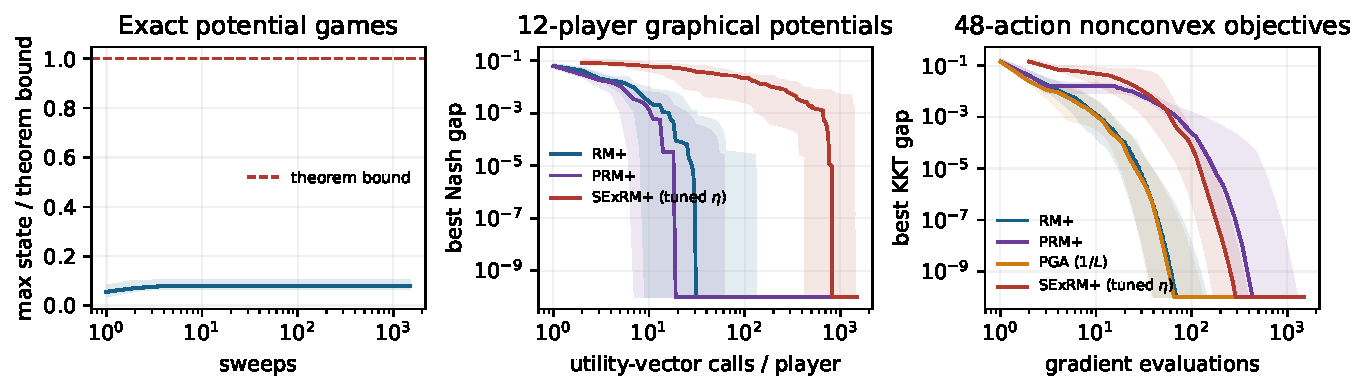
\includegraphics[width=\textwidth]{figures/diagnostics.pdf}
\caption{Mechanism and frontier baselines. Left: regret states remain below the theorem's uniform bound. Middle: alternating methods on graphical exact-potential games. Right: simplex optimization, with PGA given $1/L$. SExRM+ is favorably tuned in hindsight from the disclosed grid. Horizontal axes normalize oracle calls. Values at machine zero are displayed at $10^{-10}$.}
\label{fig:diagnostics}
\end{figure}

\section{Discussion and limitations}

The conservation law explains why the adversarial regret envelope can be loose on endogenous paths. Forward gain both measures normalized-strategy improvement and finances unnormalized-state growth. A bounded objective therefore supplies an implicit lower bound on RM+'s effective learning rate.

The product theorem requires cyclic updates because simultaneous gains need not decompose into objective changes. Its constant depends on the smallest first-positive state norm $\delta$, which can be arbitrarily small, although the one-simplex theorem is $\delta$-free. RM without per-round truncation also lacks the orthant identity. These boundaries agree with known instability outside potential structure~\citep{Farina23:Regret,Cai25:Last,Anagnostides26:Convergence}.

Appendix~\ref{app:robust} extends the charge to approximate potentials and perturbed ascent paths. Stochastic and bandit feedback remain open for RM+ because noise can make realized forward charge signed. Calibrated stochastic Frank--Wolfe methods provide complementary equilibrium and regret guarantees under bandit feedback~\citep{Dong24:Markov}.

\paragraph{Reproducibility statement.} The appendix proves all edge cases. The supplement contains fixed-seed experiments and independent audits of the identity, sharpness, smooth ascent, and product proof. Appendix~\ref{app:numerics} records protocols and tolerances.

\bibliography{references}
\bibliographystyle{iclr2027_conference}

\appendix

\section{Full details for the conservation law}
\label{app:identity}

We first justify all zero-state cases in Lemma~\ref{lem:identity}. If $r_{t-1}\ne0$, then $\langle r_{t-1},q_t\rangle\ge0$, so $R_t\ge R_{t-1}>0$. Thus a transition into the origin is impossible. If both states are zero, the two sides of~\eqref{eq:identity} vanish under the convention $x_{t+1}=x_t$. A transition from the origin to a nonzero state has $r_t=\pos{g_t}$. If $r_t$ had full support, then every coordinate of $g_t$ would be positive, contradicting $\langle x_t,g_t\rangle=0$. Therefore its support has size at most $m-1$, which is precisely the first case in the proof of Theorem~\ref{thm:charge}.

For completeness, we supply the elementary inequality used in the full-support case. Let $y\in\mathbb R_+^m$ satisfy $\|y\|_2=1$ and put $a=\min_jy[j]$. Choose a coordinate attaining $a$. Then
\begin{equation}
\|y\|_1
\le a+\sqrt{m-1}\sqrt{1-a^2}
\le a+\sqrt{m-1}
\le\sqrt{m-1}(1+a).
\end{equation}
If $y$ is the normalized new state and $z$ is the old state divided by the new norm, the no-clipping relation $\langle z,y-z\rangle=0$ yields $\langle y,z\rangle=\|z\|_2^2=\rho^2$. Since all coordinates of $y$ are at least $a$,
\begin{equation}
\rho^2=\langle y,z\rangle\ge a\|z\|_1\ge a\rho.
\end{equation}
When $\rho>0$, this gives $\rho\ge a$. The case $\rho=0$ cannot have full support, as shown above. This completes the proof without genericity assumptions.

The standard adversarial inequality quoted in Corollary~\ref{cor:variation} follows from projection onto the positive orthant:
\begin{equation}
R_t^2=\|\pos{r_{t-1}+g_t}\|_2^2
\le\|r_{t-1}+g_t\|_2^2
=R_{t-1}^2+\|g_t\|_2^2,
\end{equation}
where $\langle r_{t-1},g_t\rangle=0$. Telescoping and $\Reg_T\le R_T$ give the claim.

\section{Auxiliary smooth-optimization bounds}
\label{app:smooth}

We prove~\eqref{eq:smoothcost}. For nonzero $r,r'\in\mathbb R_+^m$ with sums $s,s'$, normalizing and adding an intermediate term gives
\begin{equation}
\left\|\frac r s-\frac{r'}{s'}\right\|_1
\le\|r-r'\|_1\left(\frac1s+\frac1{s'}\right).
\label{eq:normlip}
\end{equation}
Under~\eqref{eq:gradientrange}, every coordinate of $g_t$ lies in $[-G,G]$. A clipped decrement $q_t[a]=-r_{t-1}[a]$ can occur only when $r_{t-1}[a]\le G$, so $\|q_t\|_\infty\le G$. Hence $|s_t-s_{t-1}|\le mG$. A transition from the origin has $R_t=\|\pos{g_t}\|_2\le\sqrt mG<H$, so any update with $R_t\ge H$ has $s_{t-1}>0$. If $s_t\ge2mG$, then $s_{t-1}\ge s_t/2$. Applying~\eqref{eq:normlip}, $\|q_t\|_1\le\sqrt m\|q_t\|_2$, and $\|\cdot\|_2\le\|\cdot\|_1$ gives
\begin{equation}
\|x_{t+1}-x_t\|_2^2
\le\frac{9m}{s_t^2}\|q_t\|_2^2.
\end{equation}
If also $s_t\ge9mL$, then
\begin{equation}
\frac L2\|x_{t+1}-x_t\|_2^2
\le\frac{\|q_t\|_2^2}{2s_t}
\le\frac{D_t}{2},
\end{equation}
where the last inequality is Lemma~\ref{lem:identity}. Since $s_t\ge R_t$, the condition $R_t\ge H$ implies both required lower bounds.

It remains to justify the pre-threshold KKT charge. The positive coordinate of $g_t$ that attains~\eqref{eq:kktgap} is never clipped, so $\|q_t\|_2\ge\Gap(x_t)$. From the proof of Lemma~\ref{lem:identity},
\begin{equation}
R_t^2-R_{t-1}^2\ge\|q_t\|_2^2\ge\Gap(x_t)^2.
\end{equation}
Summing over indices before the first crossing of $H$ gives a total below $H^2$.

\section{Proof of the product-simplex theorem}
\label{app:product}

We prove Theorem~\ref{thm:product} for every finite prefix. All bounds then pass to the infinite path. Write $R_i=\|r_i\|_2$ and $s_i=\|r_i\|_1$ immediately before an activation, and add a superscript $+$ for the post-update quantities. Lemma~\ref{lem:identity} applies blockwise and gives
\begin{equation}
(R_i^+)^2-R_i^2\ge\|q_i\|_2^2,
\qquad
2s_i^+D_i=(R_i^+)^2-R_i^2+\|q_i\|_2^2.
\label{eq:productidentity}
\end{equation}
In particular, each $R_i$ is nondecreasing, $D_i\ge0$, and $\|q_i\|_2^2\le s_i^+D_i$.

We first account for low updates. For a fixed block, they form an initial prefix because $R_i$ is nondecreasing. Telescoping the first inequality in~\eqref{eq:productidentity} over this prefix gives
\begin{equation}
\sum_{\text{low updates of }i}\|q_i\|_2^2\le H_i^2.
\label{eq:lowstatebudget}
\end{equation}
Every update, low or high, also satisfies
\begin{equation}
\|x_i^+-x_i\|_2\le\frac{2\sqrt{m_i}}{\delta}\|q_i\|_2.
\label{eq:productnormalization}
\end{equation}
If both states are positive, this follows from~\eqref{eq:normlip}, $s_i,s_i^+\ge\delta$, and $\|q_i\|_1\le\sqrt{m_i}\|q_i\|_2$. If an update leaves the origin, then $q_i=r_i^+$, $\|q_i\|_2\ge\delta$, and the Euclidean diameter of the simplex is $\sqrt2\le2\sqrt{m_i}$. An update that remains at the origin does not move its retained fallback strategy. Combining~\eqref{eq:lowstatebudget} and~\eqref{eq:productnormalization},
\begin{equation}
\sum_{\rm low}\|x_i^+-x_i\|_2^2
\le\frac{4}{\delta^2}\sum_i m_iH_i^2=\frac{4A}{\delta^2}.
\label{eq:lowstrategybudget}
\end{equation}

For any block update, smoothness gives
\begin{equation}
f(x^+)-f(x)\ge D_i-\frac L2\|x_i^+-x_i\|_2^2.
\label{eq:blocksmooth}
\end{equation}
Thus the sum of objective changes over low updates is at least $-E$. If an update is high, the blockwise calculation in Appendix~\ref{app:smooth} applies with $m_i$ and the common bounds $G,L$. A transition from the origin cannot be high because $\|[g_i]_+\|_2\le\sqrt{m_i}G<H_i$. Therefore
\begin{equation}
f(x^+)-f(x)\ge D_i/2
\label{eq:producthighascent}
\end{equation}
on every high update. Telescoping all objective changes and using the range of $f$ yields
\begin{equation}
\sum_{\rm high}D_i\le2(\Delta_f+E).
\label{eq:highgainbudget}
\end{equation}

If block $i$ never becomes high, its norm remains below $H_i\le M_i$. Otherwise, immediately before its first high update its norm is at most $J_i$. All of its later updates are high. Applying Theorem~\ref{thm:charge} to that suffix and then~\eqref{eq:highgainbudget} gives
\begin{equation}
R_i\le J_i+\sqrt{m_i-1}\sum_{\text{high updates of }i}D_i\le M_i.
\label{eq:productstatebound}
\end{equation}
For high updates,~\eqref{eq:productidentity} and~\eqref{eq:productstatebound} imply
\begin{equation}
\|q_i\|_2^2\le s_i^+D_i\le\sqrt{m_i}M_iD_i\le WD_i.
\end{equation}
Combining this with~\eqref{eq:lowstatebudget} and~\eqref{eq:highgainbudget} proves
\begin{equation}
\sum_{k\ge1}S_k=\sum_{i,k}\|q_{i,k}\|_2^2
\le\sum_iH_i^2+2W(\Delta_f+E)=Q.
\label{eq:productsquarepath}
\end{equation}

We finally transfer activation gaps to a cycle endpoint. Let $z_{i,k}$ and $y_{i,k}$ be the profiles immediately before and after block $i$ updates in cycle $k$. Its activation gap $\gamma_{i,k}$ is at most $\|q_{i,k}\|_2$: a coordinate attaining the nonnegative maximum of $g_i$ is not clipped and has state increment equal to $\gamma_{i,k}$. Moreover,
\begin{equation}
\max_a\nabla_i f(z_{i,k})[a]-\langle (y_{i,k})_i,\nabla_i f(z_{i,k})\rangle
=\gamma_{i,k}-D_{i,k}\le\|q_{i,k}\|_2.
\label{eq:postgap}
\end{equation}
For fixed $p\in\Delta_{m_i}$, the function $u\mapsto\max_a u[a]-\langle p,u\rangle$ is $\sqrt2$-Lipschitz in Euclidean norm because $\|e_a-p\|_2\le\sqrt2$. Block $i$ does not move again before the endpoint $x^k$. By~\eqref{eq:productnormalization} and the disjointness of block coordinates,
\begin{equation}
\|x^k-y_{i,k}\|_2^2
\le\frac{4m}{\delta^2}\sum_{j>i}\|q_{j,k}\|_2^2
\le\frac{4m}{\delta^2}S_k.
\end{equation}
Smoothness and~\eqref{eq:postgap} therefore show that the block-$i$ endpoint gap is at most
\begin{equation}
\|q_{i,k}\|_2+\frac{2\sqrt{2m}L}{\delta}\sqrt{S_k}.
\end{equation}
Summing over blocks and using $\sum_i\|q_{i,k}\|_2\le\sqrt{nS_k}$ proves~\eqref{eq:endpointtransfer}. Among the first $K$ cycles,~\eqref{eq:productsquarepath} supplies one with $S_k\le Q/K$, proving the finite-time claim. It also implies $S_k\to0$, which proves convergence of the actual cycle-end gaps.

\section{Ordinary alternating RM+}
\label{app:nonlazy}

We prove Theorem~\ref{thm:nonlazy} by making the substitution into the argument of \citet{Anagnostides26:Convergence} explicit. Index full cycles by $t$. Let $q_{i,t}$ be player $i$'s state increment at its activation during cycle $t$. Lemma~\ref{lem:identity},~\eqref{eq:potentialidentity}, and $\|r_{i,t}\|_1\le B$ give
\begin{equation}
\sum_{t\ge1}\sum_{i=1}^n\|q_{i,t}\|_2^2
\le B\sum_{t,i}D_{i,t}
\le B\Delta_\Phi.
\label{eq:squarepath}
\end{equation}
Among the first $2K$ cycles, one disjoint adjacent pair $2k-1,2k$ therefore satisfies
\begin{equation}
\sum_i\bigl(\|q_{i,2k-1}\|_2^2+\|q_{i,2k}\|_2^2\bigr)
\le\frac{B\Delta_\Phi}{K}.
\label{eq:smallpair}
\end{equation}
Choose $K=\lceil25B\Delta_\Phi n^2m/(\delta^2\epsilon^2)\rceil$. Every state increment in the pair then has norm at most
\begin{equation}
\eta=\frac{\delta\epsilon}{5n\sqrt m}.
\end{equation}

At a player's activation, its best-response gap against the utility vector observed then is at most $\|q_{i,t}\|_\infty\le\eta$. A positive state norm is at least $\delta$, so~\eqref{eq:normlip} yields a within-activation strategy movement at most $2\sqrt m\eta/\delta$ in $\ell_1$. A player at the origin either has $q_{i,t}=0$ and does not move, or its first positive update has norm at least $\delta$. The latter is impossible in the selected pair because $\eta<\delta$. Thus the same movement bound covers every activation in the pair.

The player's own update cannot increase its gap against the opponents observed at activation because $D_{i,t}\ge0$. For a fixed own mixed action, the best-response gap changes by at most twice the $\ell_1$ change in the opponents' product distribution because every pure payoff difference lies in $[-1,1]$. The opponents move by at most $2n\sqrt m\eta/\delta$ in total during a cycle. Multiplying this movement by the gap's factor two gives the transfer cost $4n\sqrt m\eta/\delta$. Therefore every player's gap at the end of the second selected cycle is at most
\begin{equation}
\eta+\frac{4n\sqrt m\eta}{\delta}
\le\frac{5n\sqrt m\eta}{\delta}=\epsilon,
\end{equation}
where $\delta\le1$ by definition. This proves~\eqref{eq:nonlazy}. The case with no positive state is already stationary.

For the asymptotic statement,~\eqref{eq:squarepath} implies $q_{i,t}\to0$ for every player. Equation~\eqref{eq:normlip} and the positive state lower bound imply that every within-cycle strategy movement tends to zero. A state that remains at the origin does not move. Each activation-time best-response gap is at most $\|q_{i,t}\|_\infty$ and also tends to zero. Multilinearity and continuity transfer these gaps to the end-of-cycle profile, so its Nash gap converges to zero.

\section{Gain dominance and approximate potentials}
\label{app:robust}

The game proof uses only an upper bound on cumulative forward gain. The following form records the robust principle.

\begin{proposition}[Approximate gain dominance]
\label{prop:robust}
Suppose an RM+ utility path admits a scalar sequence $\Psi_t$ and errors $e_t\ge0$ such that
\begin{equation}
D_t\le\Psi_t-\Psi_{t-1}+e_t
\end{equation}
for every $t$. Then
\begin{equation}
\Reg_T\le R_0+\sqrt{m-1}
\left(\Psi_T-\Psi_0+\sum_{t=1}^Te_t\right).
\end{equation}
\end{proposition}

\begin{proof}
Sum the assumed inequalities and apply Theorem~\ref{thm:charge}.
\end{proof}

For example, if unilateral utility improvement differs from the increment of an approximate potential by at most $\zeta_t$ at activation $t$, take $e_t=\zeta_t$. Bounded cumulative approximation error preserves constant regret. A uniform per-update error $\zeta$ yields $O(1+\zeta T)$ regret, so average regret approaches an $O(\zeta)$ floor. This statement deliberately measures realized mixed deviations. Translating a particular pure-deviation definition of approximate potential into $\zeta_t$ may introduce an additional constant.

\section{Numerical proof audits}
\label{app:numerics}

The identity audit used seed $20260813$, dimensions $2$ through $32$, and 1,000 updates per dimension. It verified~\eqref{eq:identity} to residual below $1.1\times10^{-13}$ and attained normalized charge $1.000000$. The same script tested 350 alternating identical-interest games and observed a largest normalized trajectory ratio of $0.993583$. A separate audit used seed $1701$ and 5,000 normalized quadratic objectives. It verified~\eqref{eq:halfgain} with minimum sampled slack above $2.1\times10^{-7}$. The product audit used seed $20270814$, 200 random two-to-five-block quadratic-trigonometric objectives, and 300 cycles each. It checked~\eqref{eq:lowstatebudget}--\eqref{eq:endpointtransfer}, the state and global path budgets, origin transitions, and 700 separately constructed high-state updates. The smallest high-ascent slack was $4.59\times10^{-9}$, and the smallest endpoint-transfer slack was $-6.94\times10^{-18}$, within the declared $2\times10^{-9}$ tolerance.

Figure~\ref{fig:diagnostics} uses seed $20270813$, 16 instances per panel, 1,500 sweeps for the state diagnostic, and an oracle budget of 1,500 per player or simplex. A graphical-game potential is the sum of random unary terms and random pairwise terms on a 12-vertex average-degree-four graph. We scale the factors so every player's action-utility range is at most one. The smooth objectives have the form
\begin{equation}
f(x)=\tfrac12x^\top Ax+b^\top x+\frac{a}{q}\sum_{j=1}^q\sin(w_j^\top x+\phi_j),
\end{equation}
with 48 actions, $q=24$, $a=0.015$, and $\|w_j\|_2=5$. The indefinite matrix $A$ is generated so its positive eigenvalue exceeds $(a/q)\sum_j\|w_j\|_2^2$. Hence every objective has a positive-curvature direction despite the trigonometric perturbation and is nonconcave. We disclose the global smoothness bound $L=\|A\|_2+(a/q)\sum_j\|w_j\|_2^2$. SExRM+ uses Euclidean projection onto $\{r\ge0:\|r\|_1\ge1\}$. Its fixed step is selected per instance by final gap from $\{0.25,1,4\}$ for the normalized games and $\{0.25/L,1/L,4/L\}$ for the objectives. This hindsight selection favors SExRM+. PRM+ follows the public benchmark update of \citet{Tewolde26:Decision}. Metric-only evaluations are excluded. The script asserts action-range normalization, the unilateral potential identity, and positive curvature, and regenerates Figure~\ref{fig:diagnostics}. These are implementation checks, not theorem evidence.

\end{document}
